\documentclass[a4paper, 11pt]{article}
\usepackage{geometry}
\geometry{letterpaper, margin=1in}
\usepackage{amsmath}
\usepackage{amssymb}  
\usepackage{amsthm}
\usepackage{ulem} 
\usepackage{graphicx}
\graphicspath{ {images/} }

\begin{document}
%Header-Make sure you update this information!!!!
\noindent
\large\textbf{1C} \hfill \textbf{John Waczak} \\
\normalsize MTH 434 \hfill  Date: \today \\
Dr. Christine Escher \\
I took roughly \textbf{1.5 hours} to finish and type up this homework\\ 
\section*{1}
\paragraph{}a) Show that $\alpha(t)=(\sin(3t)\cos(t), \sin(3t)\sin(t), 0)$ is regular curve. 
	\begin{align*}
		\alpha'(t) &= (3\cos(3t)\cos(t)-\sin(3t)\sin(t), 3\cos(3t)\sin(t)+\sin(3t)\cos(t), 0) \\ 
			&= (\cos(2t)+2\cos(4t), 2\sin(4t)-\sin(2t), 0)\\ 
		|\alpha'(t)| &= \sqrt{(\cos(2t)+2\cos(4t))^2+(2\sin(4t)-\sin(2t))^2} \\
			&= \sqrt{4\cos(6t)+5} \\ 
		&|\sqrt{4\cos(6t)+5}| \geq 1 \quad \forall t\\
		\Rightarrow |\alpha'(t)| &\geq 0 \quad \forall t\\
		&\text{therefore}\quad \alpha(t)\quad \text{is a regular curve} \qed
	\end{align*}


b) Find the equation of the tangent line to alpha at $t=\pi/3$. 
	\begin{align*}
		T_{\pi/3}(t) &= \alpha(\pi/3)+\alpha'(\pi/3)t \\ 
		\alpha(\pi/3)&= (0, 0 ,0) \\ 
		\alpha'(\pi/3)&= (-\frac{3}{2}, -\frac{3\sqrt{3}}{2}, 0)\\ 
		\Rightarrow T_{\pi/3}(t) &= (0,0,0)+(-\frac{3}{2}, -\frac{3\sqrt{3}}{2}, 0)t\\
		&=(-\frac{3}{2}t, -\frac{3\sqrt{3}}{2}t, 0)
	\end{align*}
c) plot $\alpha(t)$.
	\begin{center}
		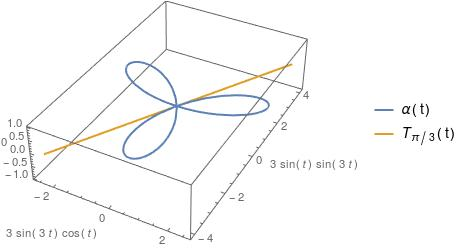
\includegraphics[scale=.75]{1c}
	\end{center}
	I have included the tangent line from part (b) as proof that it is in fact a tangent line. 
	
\section*{1.3}
	Use an improper integral to show that such a restriction has finite arc length even though it makes infinitely many loops around the origin. 
		\begin{align*}
			\gamma(t) &= c(e^{\lambda t}\cos(t), e^{\lambda t}\sin(t)) \\ 
			\gamma'(t) &= c(e^{\lambda t}(\lambda\cos(t)-\sin(t)),e^{\lambda t}(\lambda\sin(t)+\cos(t))) \\
			|\gamma'(t)| &= c\sqrt{e^{2\lambda t}((\lambda\cos(t)-\sin(t))^2+(\lambda\sin(t)+\cos(t))^2)} \\ 
			&= ce^{\lambda t}\sqrt{(\lambda\cos(t)-\sin(t)^2+(\lambda\sin(t)+\cos(t))^2} \\ 
			&= ce^{\lambda t}\sqrt{\lambda^2+1} \\ 
			\int_0^{\infty} ce^{\lambda t}\sqrt{\lambda^2+1}dt &= c\sqrt{\lambda^2+1}\Big[\frac{e^{\lambda t}}{\lambda}\Big]_0^{\infty} \\ 
			&\text{Recall that }\lambda <0, \quad \text{thus} \\ 
			&= c\sqrt{\lambda^2+1}[-\frac{1}{\lambda}] \\ 
			&= \frac{-c\sqrt{\lambda^2+1}}{\lambda} > 0
		\end{align*}	
	Thus we have shown that the logarithmic spiral has finite arc length when restricted to $[0,\infty)$ (which is nuts!)

\section*{1.16}
Let $\gamma(t)$ be a logarithmic spiral. Prove that the angle between $\gamma(t), \gamma'(t)$ is a constant function. 
	\begin{align*}
		\gamma(t) &= c(e^{\lambda t}\cos(t), e^{\lambda t}\sin(t)) \\ 
		\gamma'(t) &= c(e^{\lambda t}(\lambda\cos(t)-\sin(t)),e^{\lambda t}(\lambda\sin(t)+\cos(t))) \\
		\cos(\theta) &\equiv \frac{\langle \gamma(t), \gamma'(t)\rangle}{|\gamma(t)||\gamma'(t)|} \\ 
		|\gamma(t)| &= c\sqrt{e^{2\lambda t}\cos^2(t)+e^{2\lambda t}\sin^2(t)} \\ 
			&= ce^{\lambda t} \\ 
		|\gamma'(t)| &= ce^{\lambda t}\sqrt{\lambda^2 + 1} \\ 
		\langle \gamma(t),\gamma'(t)\rangle &= c^2e^{2\lambda t}(\lambda\cos^2(t)-\cos(t)\sin(t)+\lambda\sin^2(t)+\cos(t)\sin(t))\\ 
		&= \lambda c^2e^{2\lambda t} \\ 
		\Rightarrow \cos(\theta) &= \frac{\lambda c^2e^{2\lambda 2}}{ce^{\lambda t}ce^{\lambda t}\sqrt{\lambda^2+1}} \\ 
		&= \frac{\lambda}{\sqrt{\lambda^2+1}}\\
		\Rightarrow \theta &= \cos^{-1}(\frac{\lambda}{\sqrt{\lambda^2+1}}) = \text{constant}
	\end{align*}
	Not that because $\sqrt{\lambda^2 +1} > |\lambda|$ the argument of the inverse cosine is always between (-1, 1) and so is well defined. 
\end{document}















































